% This is samplepaper.tex, a sample chapter demonstrating the
% LLNCS macro package for Springer Computer Science proceedings;
% Version 2.20 of 2017/10/04
%
\documentclass[runningheads]{llncs}
%
\usepackage{graphicx}
% Used for displaying a sample figure. If possible, figure files should
% be included in EPS format.
%
% If you use the hyperref package, please uncomment the following line
% to display URLs in blue roman font according to Springer's eBook style:
% \renewcommand\UrlFont{\color{blue}\rmfamily}

\begin{document}
%
\pagenumbering{gobble}
\title{Fusão de informações entre imagens PolSAR e ópticas para reconhecimento de padrões}
%
%\titlerunning{Abbreviated paper title}
% If the paper title is too long for the running head, you can set
% an abbreviated paper title here
%
\pagestyle{plain}
\author{Autor: Gabrielle Cibyl da Hora \\ 
Orientador: Mauricio Marengoni} 
%
%\authorrunning{F. Author et al.}
% First names are abbreviated in the running head.
% If there are more than two authors, 'et al.' is used.
%
\institute{PPGEEC - Programa de pós-graduação em Engenharia Elétrica e Computação. 
Universidade Presbiteriana Mackenzie.\\
\email{gcibyl@gmail.com}}
%
\maketitle              % typeset the header of the contribution
%
\begin{abstract}
% AAB modificado
O projeto de pesquisa propõe a fusão de informações para reconhecimento de padrões entre imagens ópticas e canais hh, hv e vv de imagens PolSAR múltiplas visadas. Os métodos de fusão foram escolhidos a partir das referências \cite{bmf_2020} e \cite{ref_proc3}.  Será estudado a viabilidade do métodos de fusão por média, transformada wavelet discreta de multi-resolução (MR-DWT), análise de componente principal (PCA), estatísticas ROC, transformada wavelet estacionária de multi-resolução (MR-SWT) e um método multi-resolução baseado na decomposição em valores singulares (MR-SVD) com a inserção das imagens ópticas. Com o objetivo de classificar de maneira acurada as bordas vamos propor duas técnica de reconhecimento de padrões. A primeira técnica baseada em votação majoritária e a segunda técnica baseada em propriedades estatísticas das imagens. 

\keywords{PolSAR  \and Métodos de fusão \and R}
\end{abstract}
%
%
%\
\section{Introdução}

\section{Objetivos}

Este projeto de pesquisa tem como objetivo aplicar a comparação de fusão e novos métodos propostos no estudo realizado pelo Borba [1], além de dar continuidade iremos aplicar um novo canal de fusão (imagens ópticas). O principal objetivo do projeto é a aplicação das técnicas de reconhecimento de padrões para detecção de bordas sem utilizar métodos que retirem os ruídos. Como visto na introdução, o que se propõe são avanços no método de processamento de imagem PolSAR.

\section{Justificativas e motivações}
Na introdução deste projeto de pesquisa ressaltamos a importância deste tema, porém ainda podemos citar alguns tópicos que servem de motivação ao projeto:
\begin{itemize}
  \item Aplicação em estudos florestais, pesquisa mineral e detecção de derramamento de óleo.
  \item O uso da polarimetria SAR em aplicações possui necessidade de estudos mais profundos para uma compreensão interação radar-alvo, disponibilidade de dados bem calibrados, algoritmos mais robustos, etc.
  \item Processamento de imagens, pois o Radar de abertura sintética polarimétrica (PolSAR) contém ruídos do tipo speckle.
\end{itemize}


\section{Conceitos}
% AAB inserido
O projeto pode ser dividido em uma primeira etapa que consiste em encontrar bordas nos diferentes canais (imagens) e a fusão dessas bordas como segunda etapa.
\subsection{Detecção de bordas em cada canal}
 Vamos modelar as imagens PolSAR com a função de densidade de probabilidade para os canais $(hh)$, $(hv)$ e $(vv)$ usando a distribuição Wishart (PDF) descrita por
\begin{equation}
    f_{\mathbf{Z}}(\mathbf{Z};\mathbf{\Sigma_{s}},L)=\frac{L^{mL}|\mathbf{Z}|^{L-m}}{|\mathbf{\Sigma_{s}}|^{L}\Gamma_m(L)} \exp(-L\mathbf{tr}(\mathbf{\Sigma_{s}}^{-1}\mathbf{Z})), \\
\end{equation} 
onde, $\mathbf{tr}(\cdot)$ é o operador traço de uma matriz, $\Gamma_m(L)$ é uma função Gamma multivariada definida por
\begin{equation}\label{cap_acf_10}
	\Gamma_m(L)=\pi^{\frac{1}{2}m(m-1)} \prod_{i=0}^{m-1}\Gamma(L-i) \\
\end{equation}
e $\Gamma(\cdot)$ é a função Gamma. Podemos afirmar que $\mathbf{Z}$ é distribuído como uma distribuição Wishart denotando por $\mathbf{Z}\sim W(\mathbf{\Sigma_{s}}, L)$ e satisfazendo $E[\mathbf{Z}]=\mathbf{\Sigma_{s}}$. Sem perda de generalidade para o texto vamos usar o simbolo $\mathbf{\Sigma}$ em detrimento a $\mathbf{\Sigma_{s}}$ para representar a matriz de covariância associada a $\mathbf{S}$.
 
Usando a função densidade de probabilidade e o método da máxima verossimilhança vamos detectar as bordas nas imagens PolSAR. Da mesma forma temos que definir o procedimento para imagens óticas. 
\subsection{Métodos de Fusão das bordas detectadas}
\begin{itemize}
  \item Análise de componente principal (PCA).
  \item Estatística ROC.
  \item transformada wavelet discreta de multi-resolução (MR-DWT).
\end{itemize}

\subsection{Provaveis métodos de classificação}
\begin{itemize}
  \item SVM [2].
  \item Deep Learning [3].
\item Forest Classification [4].
\end{itemize}



\section{Metodologia}

\subsection{Cronograma}
\begin{figure}
\begin{center}
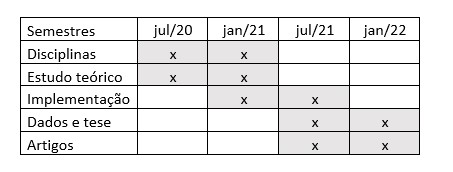
\includegraphics[scale=0.8]{cronograma.jpg}
\end{center}
\caption{A figura representa o cronograma a ser seguido para a conclusão do projeto} \label{fig1}
\end{figure}


\subsection{Estudo teórico}
\begin{itemize}
  \item Realização da pesquisa bibliográfica e estudo dos artigos obtidos.
  \item Estudo da viabilidade e decisões sobre abordagens.
\end{itemize}

\subsection{Estudo prático}

\begin{itemize}
  \item Implementação computacional das abordagens selecionadas.
  \item Validação e verificação da implementação computacional dos métodos de fusão e reconhecimento de padrões.
  \item Estudo dos dados computacional obtidos, realizando testes comparativos entre os métodos implementados.
\end{itemize}

\subsection{Resultado esperado}

\begin{itemize}
  \item Continuidade na identificação da melhor técnica de fusão propostas pelo estudo do Borba [1], que terá um artigo publicado na revista http://www.grss-ieee.org/publication-category/grsl/
  \item Otimização de reconhecimento de padrões sem aplicação de filtros nos ruídos.
\end{itemize}

\subsection{Divulgação dos resultado}

\begin{itemize}
  \item Elaboração de relatórios técnicos.
  \item Elaboração e submissão de artigos científicos para publicação em periódicos ou anuais de eventos, nacionais e internacionais.
\end{itemize}



%
% ---- Bibliography ----
%
% BibTeX users should specify bibliography style 'splncs04'.
% References will then be sorted and formatted in the correct style.
%
% \bibliographystyle{splncs04}
% \bibliography{mybibliography}
%
\begin{thebibliography}{8}
% AAB inserido
\bibitem{bmf_2020}
A. A. De Borba, M. Marengoni, A. C. Frery, Artigo por aparecer em IEEE Geoscience and Remote Sensing Society Letters (GRSL).  DOI:10.1109/LGRS.2020.3022511. 
\bibitem{ref_lncs1}
Author, F., Author, S.: Title of a proceedings paper. In: Editor,
F., Editor, S. (eds.) CONFERENCE 2016, LNCS, vol. 9999, pp. 1--13.
Springer, Heidelberg (2016). \doi{10.10007/1234567890}

\bibitem{ref_proc1}
Y. Duan, H. Duan and M. Sun, "Classification of the PolSAR Data Using Dual Classifiers," 2018 IEEE 3rd International Conference on Image, Vision and Computing (ICIVC), Chongqing, 2018, pp. 316-320, doi: 10.1109/ICIVC.2018.8492814.

\bibitem{ref_proc2}
H. Wang, F. Xu and Y. Jin, "A Review of Polsar Image Classification: from Polarimetry to Deep Learning," IGARSS 2019 - 2019 IEEE International Geoscience and Remote Sensing Symposium, Yokohama, Japan, 2019, pp. 3189-3192, doi: 10.1109/IGARSS.2019.8899902.

\bibitem{ref_proc3}
N. G. Kasapoglu, S. N. Anfinsen and T. Eltoft, "Fusion of optical and multifrequency polsar data for forest classification," 2012 IEEE International Geoscience and Remote Sensing Symposium, Munich, 2012, pp. 3355-3358, doi: 10.1109/IGARSS.2012.6350702.
\end{thebibliography}
\end{document}
